\begin{section}{Mise en place d'un bootstrapping}
\begin{subsection}{Un point sur la sécurité}
	Nous avons vu que le système cryptographique que nous étudions est IND-CPA, ce qui est le niveau de sécurité théorique que l'on veut généralement. La première question qui se pose pour le bootstrapping est de savoir si l'on garde ce niveau de sécurité.

	Le problème est que pour effectuer un déchiffrement homomorphe, il faut au moins un chiffré de la première clé secrète par la deuxième clé publique, ou, dans notre cas, un chiffré de chaque bit du secret. Il faut pouvoir s'assurer qu'un attaquant soit incapable d'en tirer des informations sur la première clé. On appelle cela la sécurité circulaire.
	
	Comme nous l'avons rappelé, le système est IND-CPA, ce qui implique que cette propriété est toujours vérifiée lorsque les deux clés sont indépendantes l'une de l'autre. Il suffit donc de générer les clés indépendamment les unes des autres pour s'assurer d'avoir le niveau de sécurité désiré.
\end{subsection}
\begin{subsection}{Un premier découpage}
	Afin de pouvoir effectuer un bootstrapping à partir de l'algorithme de déchiffrement \textbf{Dec}, nous allons avoir besoin de l'exprimer uniquement à partir d'opérations \textbf{NAND} sur des 0 et des 1.
	
	La première clé secrète est un vecteur d'éléments de $\ZZq$, pas de \{0,1\}, ce qui signifie que pour pouvoir l'utiliser dans le bootstrapping, on est contraint de se servir des chiffrés de chaque bit de chaque élément de la clé.

	Pour cela, on considère qu'à tous les éléments de $\ZZq$ est associé une liste de $l-1$ éléments contenant son écriture en binaire.

\begin{lstlisting}
decrypt(C) :
	trouver $1 \leq i \leq l$ tel que $q/4 \leq 2^i < q/2$
	calculer $a = C_i \cdot \vec{v}$
	retourner $|\frac{a}{\vec{v}_i}|$
\end{lstlisting}

Notons que:

\begin{align*}
	C_i \cdot \vec{v} &= \sum_{j=0}^N C_{i,j} v_j \\
	&= \sum_{j=0}^N \sum_{k=0}^l \left( C_{i,j,k} 2^k \right) v_j \\
	&= \sum_{j=0}^N \sum_{k=0}^l C_{i,j,k} (2^k v_j)
\end{align*}

	Or, même lorsque l'algorithme se fait homomorphiquement, les valeurs $C_{i,j,k} \in \{ 0,1 \}$ sont connues. On réduit donc le problème de calculer un produit scalaire à celui de faire la somme d'au plus $l * N$ vecteurs constitués de 0 et de 1.

	Nous allons maintenant voir comment décrire l'algorithme uniquement avec des portes \textbf{NAND}, et majorer la profondeurs en \textbf{NAND} de l'algorithme final.

	Comme nous utiliserons aussi les portes logiques \path{NO}, \path{AND}, \path{OR} et \path{XOR}, notons que:
\begin{itemize}
\item \path{NO}$(a) = \overline{a}$ se fait en un \textbf{NAND};
\item \path{AND}$(a, b) = a \land b$ se calcule en deux \textbf{NAND} et est de
	profondeur 2;
\item \path{OR}$(a, b) = a \lor b$ se fait en trois \textbf{NAND} et est de
	profondeur 2;
\item \path{XOR}$(a, b) = a \oplus b$ se calcule en six \textbf{NAND} et est de
	profondeur 4.
\end{itemize}

\end{subsection}
\begin{subsection}{Sommer des vecteurs avec une profondeur en NAND minimale}

	Nous voulons pouvoir sommer homomorphiquement $nb$ nombres vus comme des listes de taille $s$ dont les éléments sont des chiffrés de 0 ou de 1 en minimisant la profondeur de NAND requise. 

	Pour cela, nous allons tout d'abord étudier deux opérations simples sur des listes.


\vspace{0.3cm}
\noindent
\textbf{basic\_sum : addition classique de deux listes :}
\paragraph{}
	Il s'agit de l'algorithme naïf de somme de deux nombres binaire, commençant par les bits de poids faible puis remontant vers les bits de poids plus élevés en conservant des retenues, sauf celle qui \og sort \fg des listes. On l'appellera ici \textbf{basic\_sum}. Soient 
\[ A = \sum_{i=0}^{s-1} a_i 2^i \quad B = \sum_{i=0}^{s-1} b_i 2^i\]
que l'ont veux sommer. La somme
\[C =\sum_{i=0}^{s-1} c_i 2^i\]
est alors définie par :
	
\begin{figure}[!h]
\begin{lstlisting}
$r_{-1}$ = 0
for $i$ in range($s$):
	$c_i$ = $a_i \oplus b_i \oplus r_{i-1}$
	$r_i$ = $(a_i \land b_i) \lor (r_{i-1} \land (a_i \lor b_i))$
\end{lstlisting}
\end{figure}

	Le problème de cette méthode est que la profondeur de NAND nécessaire explose du fait que la formule exprimant $c_{s-1}$ dépend de $a_0$ et $b_0$, et ce à cause de la récursivité du calcul des $r-i$.

	Calculer $c_i$ peut se faire en n'utilisant la retenue que pour un $\oplus$, ce qui n'ajoute que 4 à la profondeur en \textbf{NAND} du calcul. $r_i$ est calculé en appliquant un \path{AND} et un \path{OR} à $r_{i-1}$, ce qui ajoute aussi 4 à la profondeur. $r_0 = a_0 \land b_0$ et peut donc être trouvé avec une profondeur de 2 \textbf{NAND}.
	
	On obtient alors la proposition suivante :
\begin{prop}
	L'algorithme \textbf{basic\_sum} nécessite une profondeur de $4*s - 2$ \textbf{NAND}.
\end{prop}


\vspace{0.3cm}
\noindent
\textbf{reduced\_sum :}
\paragraph{}

	Soient 
\[A = \sum_{i=0}^{s-1} a_i 2^i, \quad B = \sum_{i=0}^{s-1} b_i 2^i, \quad C = \sum_{i=0}^{s-1} c_i 2^i. \]
\textbf{reduced\_sum} va créer deux nombres qu'on nomme $X = \sum_{i=0}^{s-1} x_i 2^i$  et $Y = \sum_{i=0}^{s-1} y_i 2^i$ tels que $A + B + C = X + Y$.

	Ils se construisent ainsi, avec la convention que pour tout vecteur v, $v_i = 0 \  \forall \, i \not\in \llbracket 0, s-1 \rrbracket$ :
\begin{figure}[!h]
\begin{lstlisting}
for $i$ in range($s$):
	$x_i$ = $a_i \oplus b_i \oplus c_i$
	$y_i$ = $\overline{(\overline{a_{i-1}} \land \overline{b_{i-1}}) \oplus
	(\overline{b_{i-1}} \land \overline{c_{i-1}}) \oplus
	(\overline{a_{i-1}} \land \overline{c_{i-1}})}$
\end{lstlisting}
\end{figure}

	On remarque qu'ici, les coordonnées des résultats ne dépendent que des coordonnées voisines. La profondeur totale en NAND sera donc le max de la profondeur du calcul de $x_i$ et de celle du calcul de $y_i$.
	
	Calculer $x_i$ consiste en deux $\oplus$ successifs dont le deuxième utilise le résultat du premier. La profondeur en \textbf{NAND} est donc de 8. La profondeur maximale du calcul de $y_i$ est celle des éléments impliqués dans deux $\oplus$. Ces éléments subissent donc deux \path{NO}, un \path{AND} et deux \path{XOR}, atteignant ainsi une profondeur de 12 \textbf{NAND}.

\begin{prop}
	L'algorithme \textbf{reduction\_sum} nécessite une profondeur de $12$ \textbf{NAND}.
\end{prop}

	On comprend donc que pour sommer plusieurs listes, nous avons tout intérêt à utiliser \textbf{reduced\_sum} jusqu'à qu'il ne reste plus que deux listes, puis à utiliser \textbf{basic\_sum}, mais comment organiser ces "additions" de façon à minimiser la profondeur totale ?

\vspace{0.3cm}
\noindent
\textbf{organiser la somme des $nb$ listes :}
\paragraph{}
	L'algorithme naïf consisterai dans le premier cas à appliquer \textbf{basic\_sum} à deux listes puis à l'appliquer à chaque fois au résultat de la dernière somme avec une autre liste. Les deux variables additionnées lors de la première addition serait impliquées dans chacune	des $nb-1$ opérations et la profondeur en \textbf{NAND} serait donc de $(nb-1)(4 s - 2)$.
	
\paragraph{}
	Dans le cas de \textbf{reduced\_sum}, l'algorithme naïf consisterai en : appliquer \textbf{reduced\_sum} à trois des listes à additionner, puis en choisir une autre et appliquer \textbf{reduced\_sum} à cette dernière accompagnée des deux listes précédemment retournée par \textbf{reduced\_sum} et ainsi de suite, jusqu'à ce qu'il ne reste plus de liste à ajouter au dernier résultat. On y applique alors \textbf{basic\_sum}. On atteint ainsi une profondeur de $12(nb - 2) + 4 s- 2 = 4(3nb + s) - 26$ \textbf{NAND}.
	
\paragraph{}
	Les additions peuvent cependant être bien mieux ordonnées :
	
	Par exemple, en visualisant l'organisation comme un arbre, un arbre équilibré réduit au maximum la profondeur et permet à de sommer les $nb$ listes en utilisant uniquement \textbf{basic\_sum} avec une profondeur en \textbf{basic\_sum} de $\log_2(nb)$. On obtient donc une profondeur en \textbf{NAND} en $\mathcal{O}(\log(nb) * (4s - 2)) = \mathcal{O}(s * \log(nb))$ et non plus en $\mathcal{O}(s * nb)$.

	Si l'on construit un équivalent pour \textbf{reduced\_sum}, toujours en terminant par un \textbf{basic\_sum}, on obtient une profondeur en \textbf{NAND} en $\mathcal{O}(\log(nb) + s)$.

\begin{prop}
	Il est possible de sommer $\text{nb}$ vecteurs de $s$ éléments avec une profondeur de $4s + 36\log_3(nb) -22$ \textbf{NAND}.
\end{prop}

\begin{proof}
	Soit $p \geqslant 3$ tel que $3^{p-1} < nb \leqslant 3^{p}$.
	
	En réunissant les listes à notre disposition par groupes de 3 et en leur appliquant \textbf{reduced\_sum}, puis en recommançant deux fois on se retrouve avec au plus $8 * 3^{p-3} < 3^{p-1}$ listes à sommer.
	
	On peut donc se ramener à $nb' \leqslant 9$ avec une profondeur en \textbf{reduced\_sum} de $3(p - 2)$.
	
	De là, on peut calculer la somme totale avec une profondeur de quatre \textbf{reduced\_sum} et un \textbf{basic\_sum} :

\center
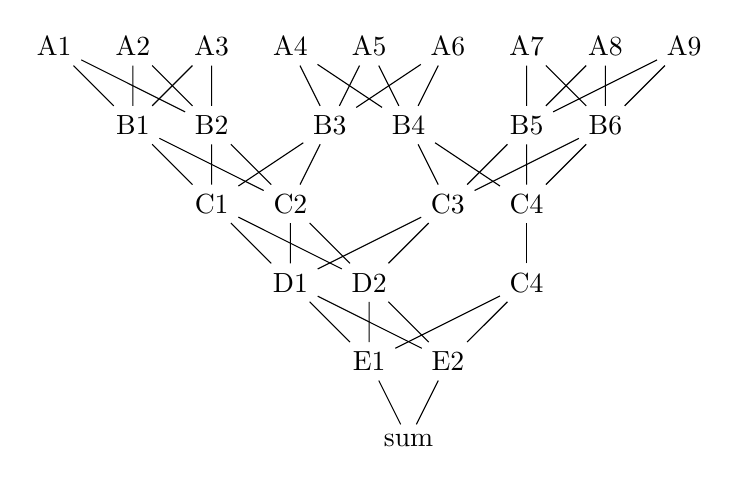
\begin{tikzpicture}
\node (A1) at (0,0) {A1};
\node (A2) at (1,0) {A2};
\node (A3) at (2,0) {A3};
\node (A4) at (3,0) {A4};
\node (A5) at (4,0) {A5};
\node (A6) at (5,0) {A6};
\node (A7) at (6,0) {A7};
\node (A8) at (7,0) {A8};
\node (A9) at (8,0) {A9};

\node (B1) at (1,-1) {B1};
\node (B2) at (2,-1) {B2};
\node (B3) at (3.5,-1) {B3};
\node (B4) at (4.5,-1) {B4};
\node (B5) at (6,-1) {B5};
\node (B6) at (7,-1) {B6};

\draw (B1) --(A1) --(B2);
\draw (B1) --(A2) --(B2);
\draw (B1) --(A3) --(B2);
\draw (B3) --(A4) --(B4);
\draw (B3) --(A5) --(B4);
\draw (B3) --(A6) --(B4);
\draw (B5) --(A7) --(B6);
\draw (B5) --(A8) --(B6);
\draw (B5) --(A9) --(B6);

\node (C1) at (2,-2) {C1};
\node (C2) at (3,-2) {C2};
\node (C3) at (5,-2) {C3};
\node (C4) at (6,-2) {C4};

\draw (C1) --(B1) --(C2);
\draw (C1) --(B2) --(C2);
\draw (C1) --(B3) --(C2);
\draw (C3) --(B4) --(C4);
\draw (C3) --(B5) --(C4);
\draw (C3) --(B6) --(C4);

\node (D1) at (3,-3) {D1};
\node (D2) at (4,-3) {D2};
\node (D3) at (6,-3) {C4};

\draw (D1) --(C1) --(D2);
\draw (D1) --(C2) --(D2);
\draw (D1) --(C3) --(D2);
\draw (D3) --(C4);

\node (E1) at (4,-4) {E1};
\node (E2) at (5,-4) {E2};

\draw (E1) --(D1) --(E2);
\draw (E1) --(D2) --(E2);
\draw (E1) --(D3) --(E2);

\node (sum) at (4.5,-5) {sum};

\draw (E1) --(sum) --(E2);
\end{tikzpicture}

	On obtient ainsi une profondeur totale en \textbf{NAND} de $4 s - 2 + 12(3p - 2) = 4s + 36p -22$. Or, par définition, $p = \lceil \log_3(nb) \rceil$ donc on a bien une profondeur en \textbf{NAND} de $4s + 36\log_3(nb) -22$.
\end{proof}

\end{subsection}
\begin{subsection}{Prendre la valeur absolue dans $\ZZq$}
	Rappelons que la valeur absolue d'un élément $x\in \ZZq$ est par définition la valeur absolue de son représentant dans $\rrbracket -q/2, q/2\rrbracket$. 
	
	Dans notre situation, $q = 2^l$ et nous représentons $a\in \ZZq$ par une liste de taille\footnote{Pour des raisons techniques, il est en fait représenté par une liste de taille $l$, mais nous ne faisons alors pas attention au dernier bit} $l-1$, le bit de poids faible étant à gauche. Autrement dit :
\[ a = [a_0, ..., a_{l-1}] \quad \text{pour représenter } a = \sum_{i=0}^{l-1} a_i 2^i\]

	On peut alors calculer en binaire la valeur absolue de $a$ ainsi :

\vspace{0.5cm}
\begin{lstlisting}
if $a_{l-1} = 0$: 
	# on a $a < q/2$
	return $a$
else:
	# on a $a < q/2$, alors $|a - q| = \left( (2^l - 1) - a + 1 \right)$
	$a$ = [NOT($a_i$) for $i$ in range($l$)]
	return basic_sum($a$, $1$)
\end{lstlisting}

	Toutefois, il n'est pas possible de faire de conditions homomorphiquement avec ce système, aussi, afin de pouvoir l'écrire homomorphiquement, on va en fait considérer le code suivant:

\vspace{0.5cm}
\begin{lstlisting}
$b$ = basic_sum([NOT($a_i$) for $i$ in range($l$)], 1)
return [($a_{l-1} \land a_i) \lor (\overline{a_{l_1}} \land b_i)$  for $i$ in range($l$)]
\end{lstlisting}

	On peut alors utiliser les comptes déjà fait, notamment concernant la profondeur en \textbf{NAND} de \textbf{basic\_sum}, pour conclure :

\begin{prop}
	En conservant nos conventions pour la représentation des données, prendre la valeur absolue d'un élément $a\in \ZZq$ demande une profondeur de $4s + 2$ \textbf{NAND}.
\end{prop}
\end{subsection}

	En additionnant nos différents comptes, on peut alors conclure :

\begin{prop}
On peut effectuer l'algorithme \textbf{Dec} avec une profondeur de
RESULTAT NAND.
	On peut effectuer l'algorithme \textbf{Dec} avec une profondeur de RESULTAT NAND.
\end{prop}
	



\end{section}
